% Created 2022-05-15 Sun 13:43
% Intended LaTeX compiler: pdflatex
\documentclass[aspectratio=169, 10pt]{beamer}
\usepackage[utf8]{inputenc}
\usepackage[T1]{fontenc}
\usepackage{graphicx}
\usepackage{longtable}
\usepackage{wrapfig}
\usepackage{rotating}
\usepackage[normalem]{ulem}
\usepackage{amsmath}
\usepackage{amssymb}
\usepackage{capt-of}
\usepackage{hyperref}
\usepackage{color}
\usepackage{listings}
\usepackage[english]{babel}
\usepackage[utf8]{inputenc}
\usepackage{roboto}
\usepackage[light,scaled=0.85]{roboto-mono}
\usepackage[T1]{fontenc}
\usepackage{codebeam}
\usepackage{tikz}
\usepackage{adjustbox}
\usetikzlibrary{arrows,automata,positioning}
\usetikzlibrary{overlay-beamer-styles}
\usepackage{pgfpages}
\usepackage{listings}

\lstset{
  extendedchars=true,
  escapeinside={\#@}{\^^M},
  literate=
  {á}{{\'a}}1 {é}{{\'e}}1 {í}{{\'i}}1 {ó}{{\'o}}1 {ú}{{\'u}}1
  {Á}{{\'A}}1 {É}{{\'E}}1 {Í}{{\'I}}1 {Ó}{{\'O}}1 {Ú}{{\'U}}1
  {à}{{\`a}}1 {è}{{\`e}}1 {ì}{{\`i}}1 {ò}{{\`o}}1 {ù}{{\`u}}1
  {À}{{\`A}}1 {È}{{\'E}}1 {Ì}{{\`I}}1 {Ò}{{\`O}}1 {Ù}{{\`U}}1
  {ä}{{\"a}}1 {ë}{{\"e}}1 {ï}{{\"i}}1 {ö}{{\"o}}1 {ü}{{\"u}}1
  {Ä}{{\"A}}1 {Ë}{{\"E}}1 {Ï}{{\"I}}1 {Ö}{{\"O}}1 {Ü}{{\"U}}1
  {â}{{\^a}}1 {ê}{{\^e}}1 {î}{{\^i}}1 {ô}{{\^o}}1 {û}{{\^u}}1
  {Â}{{\^A}}1 {Ê}{{\^E}}1 {Î}{{\^I}}1 {Ô}{{\^O}}1 {Û}{{\^U}}1
  {œ}{{\oe}}1 {Œ}{{\OE}}1 {æ}{{\ae}}1 {Æ}{{\AE}}1 {ß}{{\ss}}1
  {ç}{{\c c}}1 {Ç}{{\c C}}1 {ø}{{\o}}1 {å}{{\r a}}1 {Å}{{\r A}}1
  {ñ}{~n}1
  {€}{{\EUR}}1 {£}{{\pounds}}1
  {¿}{{?`}}1 {¡}{{!`}}1 {‘}{`}1 {’}{'}1
  {·}{.}1
}

%% AH: I have tried to follow the emacs color theme jsc-light2
\usepackage{xcolor}
\definecolor{commentcolor}{rgb}{.804,0,0}
\definecolor{builtincolor}{rgb}{.855, .439, .839}
\definecolor{keywordcolor}{rgb}{.608,.19,1}
\definecolor{stringcolor}{rgb}{0,.545,0}
\definecolor{typecolor}{rgb}{0,0,.502}
\definecolor{atomcolor}{rgb}{1,.204,.70}
\definecolor{variablecolor}{rgb}{.545,.352,.17}
\definecolor{macrocolor}{rgb}{.628,.125,.94}

\lstdefinelanguage{elixir}{
    morekeywords={
      after,
      alias,
      and,
      case,
      catch,
      cond,
      def,
      defimpl,
      defmacro,
      defmacrop,
      defmodule,
      defoverridable,
      defp,
      defprotocol,
      defstruct,
      do,
      else,
      end,
      false,
      fn,
      for,
      if,
      import,
      in,
      nil,
      not,
      or,
      quote,
      raise,
      receive,
      require,
      rescue,
      true,
      try,
      unless,
      use,
      when,
      with,
      unquote,
      command,
      state,
      invariants,
      pre,
      args,
      post,
      next,
      call
    },
    emph={iex},
    alsoletter={:},
    sensitive=true,
    morecomment=[l]{\#},
    morecomment=[n]{/*}{*/},
    morecomment=[n]{@doc\ "}{"},
    morecomment=[n]{@doc\ """}{"""},
    string=[b]",
    morestring=[b]',
    showstringspaces=false
}

\lstdefinestyle{color}{
  identifierstyle=\idstyle,
  commentstyle=\itshape\color{commentcolor},
  keywordstyle=\bfseries\color{keywordcolor},
  stringstyle=\color{stringcolor},
  emphstyle=\bfseries
}

\lstdefinestyle{nocolor}{
  identifierstyle=\itshape,
  commentstyle=\itshape,
  keywordstyle=\bfseries,
  stringstyle=,
  emphstyle=\itshape
}

%% Idea for changing identifier colors taking into account :, @ and _
%% Inspiration:
%% - https://tex.stackexchange.com/questions/4198/emphasize-word-beginning-with-uppercase-letters-in-code-with-lstlisting-package)
%% - https://tex.stackexchange.com/questions/497182/highlight-all-identifiers-starting-with-an-underscore/497212#497212
%% - And package xstring
\usepackage{xstring}
\makeatletter
\newcommand*\idstyle{\expandafter\id@style\the\lst@token\relax}
\def\id@style#1#2\relax{%
  \edef\@lowline{\expandafter\noexpand\csname lst@um_\endcsname}%
  \ifcat#1%
    \relax%
  \else%
    \IfBeginWith{#1}{\@lowline}{% starts _
      \itshape\color{commentcolor}%
    }{%
      \IfBeginWith{#1}{:}{\color{atomcolor}}{}% starts :
      \IfEndWith{#2}{:}{\color{atomcolor}}{}% ends :
      \ifnum`#1=64% starts @
        \bfseries\color{builtincolor}%
      \else%
        \ifnum`#1=\uccode`#1% starts uppercase
          \itshape\color{typecolor}%
        \else%
          % default style
        \fi%
      \fi%
    }%
  \fi%
}
\makeatother

\lstdefinestyle{display}{style=color,basicstyle=\footnotesize\ttfamily}
\lstset{morekeywords={state, command, invariants}}
\usetheme{default}
\author{Luis Eduardo Bueso de Barrio}
\date{\today}
\title{Improve your tests with Makina}
\hypersetup{
 pdfauthor={Luis Eduardo Bueso de Barrio},
 pdftitle={Improve your tests with Makina},
 pdfkeywords={},
 pdfsubject={},
 pdfcreator={Emacs 28.1 (Org mode 9.5.2)}, 
 pdflang={English}}
\begin{document}

\texturetheme

\setbeamertemplate{title page}{
    \begin{columns}
      \begin{column}{0.55\textwidth}
        \center
        \includegraphics[width=\textwidth]{./template/logo-white}
      \end{column}
      \begin{column}{0.40\textwidth}
        \flushright
            {\Huge STOCKHOLM}

            \vspace{0.2cm}

            {\large HYBRID CONFERENCE}

            \vspace{1cm}

            {\Large \texttt{Improve your tests with Makina}}

            \vspace{1cm}

            Luis Eduardo Bueso de Barrio

            \vspace{0.5cm}

            \texttt{May 20 | 2022}
      \end{column}
    \end{columns}
}

\maketitle

\whitetheme

\section{Introduction}
\label{sec:org0c60e7c}

\begin{frame}[label={sec:orgb48492f}]{The problem}
\begin{columns}
\begin{column}{0.48\columnwidth}
\begin{center}
\begin{tabular}{rrrr}
files & blank & comment & code\\
\hline
4 & 760 & 383 & 4513\\
\end{tabular}
\end{center}
\end{column}

\begin{column}{0.48\columnwidth}
\begin{center}
\begin{tabular}{rrrr}
files & blank & comment & code\\
\hline
18 & 500 & 408 & 1692\\
\end{tabular}
\end{center}
\end{column}
\end{columns}
\end{frame}


\begin{frame}[label={sec:orgf611dc7},fragile]{Introduction to PBT}
 \begin{columns}
\begin{column}{0.48\columnwidth}
Writing unit-tests is hard and time-consuming:

\lstset{language=elixir,label= ,caption= ,captionpos=b,numbers=none,style=display}
\begin{lstlisting}
reverse([]) == []
reverse([1]) == [1]
reverse([1 ,2]) == [2 ,1]
...
\end{lstlisting}

Property-Based Testing (PBT) philosophy:

\begin{quote}
Don't write tests, generate them.
\end{quote}

A test execution in PBT consists of:
\begin{enumerate}
\item Data generation.
\item Property checking.
\item An shrinking strategy (if the property doesn't hold).
\end{enumerate}
\end{column}

\begin{column}{0.48\columnwidth}
A property:

\lstset{language=elixir,label= ,caption= ,captionpos=b,numbers=none,style=display}
\begin{lstlisting}
forall list <- list() do
  list == reverse(reverse(list))
end
\end{lstlisting}

In each test:
\begin{enumerate}
\item \texttt{list()} generates a random list:
\lstset{language=elixir,label= ,caption= ,captionpos=b,numbers=none,style=display}
\begin{lstlisting}
[8 ,10 ,6] ...
\end{lstlisting}

\item Checks the property:
\lstset{language=elixir,label= ,caption= ,captionpos=b,numbers=none,style=display}
\begin{lstlisting}
[8, 10, 6] == reverse(reverse([8, 10, 6]))
\end{lstlisting}

\item If the property doesn't hold returns a counter-example.
\end{enumerate}
\end{column}
\end{columns}
\end{frame}


\begin{frame}[label={sec:org0b5bef9},fragile]{Testing \emph{stateful} programs}
 \begin{columns}
\begin{column}{0.38\columnwidth}
Imagine a simple counter:
\begin{center}
\begin{tabular}{l l c}
Command & Returns\\
\hline
\texttt{start/1} & \texttt{:ok} \(\vert\) \texttt{:error}\\
\texttt{stop/0} & \texttt{:ok} \(\vert\) \texttt{:error}\\
\texttt{inc/0} & \texttt{:ok}\\
\texttt{get/0} & \texttt{integer()}\\
\end{tabular}
\end{center}


Unit test:

\lstset{language=elixir,label= ,caption= ,captionpos=b,numbers=none,style=display}
\begin{lstlisting}
:ok = start(0)
:ok = inc()
1   = get()
:ok = stop()
\end{lstlisting}
\end{column}

\begin{column}{0.58\columnwidth}
This test can be represented:
\begin{figure}
\begin{center}
  \begin{adjustbox}{max width=\textwidth}
    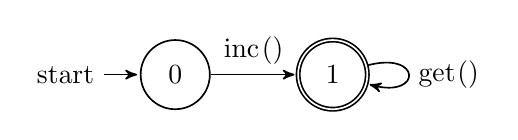
\begin{tikzpicture}[->,>=stealth',shorten >=1pt,auto,node distance=2cm,semithick]

      \node[initial,state] (0) {$0$};

      \node[state] (1) [right of=0] {$1$};
      \path[] (0) edge node {\lstinline{inc()}} (1);

      \path[] (1) edge [loop right] node {\lstinline{get()}} (1);

      \node[state, accepting] (2) [right of=0] {};
    \end{tikzpicture}
  \end{adjustbox}
\end{center}
\end{figure}

To successfully test this program we need to:
\begin{itemize}
\item Generate sequences of commands.
\item An internal state to track the changes in the program.
\item A way to interact with the program under test.
\end{itemize}
\end{column}
\end{columns}
\end{frame}


\begin{frame}[label={sec:org0a5f3d3},fragile]{PBT of \emph{stateful} programs}
 \begin{columns}
\begin{column}{0.58\columnwidth}
Basic property of \emph{stateful} programs:
\lstset{language=elixir,label= ,caption= ,captionpos=b,numbers=none,style=display}
\begin{lstlisting}
forall cmds <- commands(Counter) do
  :ok == run_commands(Counter, cmds)
end
\end{lstlisting}

where:
\begin{itemize}
\item \texttt{commands/1} generates sequences commands:
\lstset{language=elixir,label= ,caption= ,captionpos=b,numbers=none,style=display}
\begin{lstlisting}
[start(0), inc(), get(), stop()]
...
\end{lstlisting}

\item \texttt{run\_commands} executes the generated sequence.
\end{itemize}
\end{column}


\begin{column}{0.38\columnwidth}
\begin{figure}
\begin{center}
  \begin{adjustbox}{max width=\textwidth}
    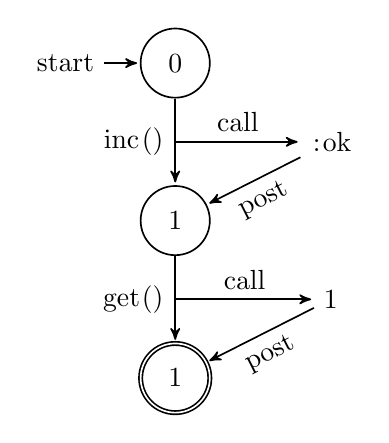
\begin{tikzpicture}[->,>=stealth',shorten >=1pt,auto,node distance=2cm,semithick]

      \node[initial,state] (i0) {$0$};
      \node[state] (i1) [below of=i0] {$1$};
      \node[state] (i2) [below of=i1] {$1$};

      \path []
      (i0) edge node (inc)  [left] {\lstinline{inc()}} (i1)
      (i1) edge node (get)  [left] {\lstinline{get()}} (i2);

      % first call
      \node[] (inc_res)  [right of=inc, xshift=0.5cm] {\lstinline{:ok}};
      \path[] (inc) edge node (inc_call)  [sloped] {\lstinline{call}} (inc_res);
      \path[](inc_res)  edge node (inc_post) [sloped, below] {\lstinline{post}} (i1);

      % second call
      \node[] (get_res)  [right of=get, xshift=0.5cm] {\lstinline{1}};
      \path[] (get)  edge node (get_call)  [sloped] {\lstinline{call}} (get_res);
      \path[] (get_res)  edge node (get_post) [sloped, below] {\lstinline{post}} (i2);

      \node[state, accepting] (i3) [below of=i1]{};
    \end{tikzpicture}
  \end{adjustbox}
\end{center}
\end{figure}
\end{column}
\end{columns}
\end{frame}


\begin{frame}[label={sec:org2cb6ddc},fragile]{Introduction to Makina}
 \texttt{Makina} is a DSL to write PBT state machines.
\begin{itemize}
\item Fully compatible with \texttt{Erlang QuickCheck} and \texttt{PropEr}.
\item 
\end{itemize}
\end{frame}


\begin{frame}[label={sec:orgaef6427}]{Ethereum Blockchain}
\end{frame}

\section{Makina features}
\label{sec:org13fd8f6}

\begin{frame}[label={sec:org2afa1f8},fragile]{Mining blocks}
 \lstset{language=elixir,label= ,caption= ,captionpos=b,numbers=none,style=display}
\begin{lstlisting}
defmodule Blocks do
  use Makina, implemented_by: Etherex

  state height: 0

  invariants non_neg_height: height >= 0

  command block_number() do
    post {:ok, height} == result
  end

  command mine() do
    call Etherex.Time.mine()
    next height: height + 1
  end
end
\end{lstlisting}
\end{frame}

\begin{frame}[label={sec:orgbbc06d6}]{Consulting accounts}
\end{frame}

\begin{frame}[label={sec:orgeed3946}]{Generating transactions}
\end{frame}

\begin{frame}[label={sec:orgb100e30}]{An abstract model for contracts}
\end{frame}

\begin{frame}[label={sec:org0d7ef1f}]{A basic model to test a contract}
\end{frame}
\end{document}